\section{Kinematics for the Da vinci robot}
This section is covering the derivation of one hand of the da Vinci robot.

It can be seen on \figref{fig:da_hand_kino}, at the end of the hand there is marked a stationary point. This point is seen as the reference point for the hand. The hand has three DOF where two of them is rotations and the last one is the translation. Both rotations can be put at the stationary point due to the fact that each rotation will not translate the stationary point of the hand. The translation is handling the position of the end-effector in respect to the reference point, where the distance is marked as $d_3$ on \figref{fig:da_hand_kino}.

The DH parameters for the da Vinci hand can be seen on \tabref{tab:DH_notation_hand} as two rotations and one translation.

\begin{figure}[H]
		\centering
		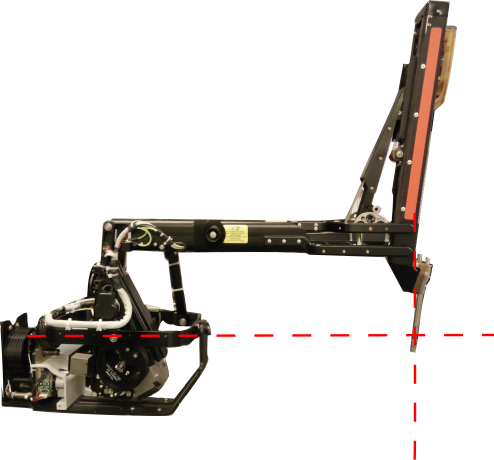
\includegraphics[width=0.6\linewidth]{Hand_davinci_robot.png}
		\caption{The da Vinci hand. The cross section shows the stationary reference for the hand. The blue arrows illustrate the two rotations in in the reference point. The green arrow is the movement of the Endo-Wrist and $d_3$ is the distance between the reference and end-effector.}
		\label{fig:da_hand_kino}
\end{figure}


\begin{table}[H]
\centering
\begin{tabular}{|l|l|l|l|l|}
	\hline
 	$j_i$ 	  & $a_i$    & $d_i$ & $\alpha_i$ 		 & $\theta_i$ 			   	 \\ \hline
 	1  	  	  &  $0$     & $0$ 	 & $-\frac{\pi}{2}$	 		 & $q_1$ 			    	 \\ \hline
 	2  		  &  $0$   	 & $0$ 	 & $ \frac{\pi}{2}$ 	 & $\frac{\pi}{2}+q_2$ 		 \\ \hline
 	3 	 	  &  $0$	 & $d_3$ & $0$ 		 		 & $0$ 					 \\ \hline
\end{tabular}
\caption{The DH notations for the da Vinci hand.}
\label{tab:DH_notation_hand}
\end{table}


